\chapter{Cinématique du point}
\label{chapter1}

\paragraph{}\textit{La mécanique est la science du mouvement des corps. Comment la Terre tourne-t-elle autour du Soleil ? Comment les oiseaux volent-ils ? Comment les roches sédimentent-elles ? Pourquoi certains acides aminés s'attirent-ils ? Voilà autant de questions auxquelles la mécanique prétend pouvoir répondre. Dans ce cours nous allons aborder les bases de la mécanique classique afin de développer votre intuition physique sur cet aspect du monde qui nous entoure quotidiennement.}

\paragraph{}\textit{Pour commencer, nous allons nous intéresser à une branche spécifique de la mécanique : la cinématique. Celle-ci s'intéresse à la description du mouvement des objets, sans s'intéresser aux causes de celui-ci. C'est la fondation essentielle nécessaire à la compréhension du reste, car pour pouvoir comprendre le mouvement, il faut d'abord être capable de le décrire.} 

\paragraph{Objectifs du chapitre}

\begin{itemize}
	
	\item Définir l'approximation ponctuelle en mécanique.
	
	\item Repérer un point dans l'espace dans différentes dimensions et grâce à différents systèmes de coordonnées.
	
	\item Être familier avec la notion de référentiel.	
	
	\item Décrire une trajectoire dans l'espace via la position, la vitesse et l'accélération.
	
	\item Caractériser des mouvements modèle simples.
	
\end{itemize}

\section{L'approximation ponctuelle en mécanique}

\paragraph{}En mécanique classique, la plupart du temps, les objets dont on souhaite décrire le mouvement sont des solides. Par définition, un solide est un système matériel dont les points restent à distance constante les uns des autres. Pour décrire totalement un solide on a donc besoin de six paramètres : la position du centre de gravité (donc trois coordonnées) et trois angles d'orientation (voir \autoref{fig:anglesolide}).

\begin{figure}[h]
	\centering
	\includegraphics[width=0.8\textwidth]{Chapitre1/Figures/angles_solide.png}
	\caption{Repérage d'un solide}
	\label{fig:anglesolide}
\end{figure}

\paragraph{}Cette quantité de paramètres rend l'étude riche mais potentiellement complexe sans raison. En effet, dans la plupart des cas, on s'intéresse uniquement à la position du centre de gravité du solide (une sorte de position moyenne) et son évolution au cours du temps. Pour simplifier l'étude du mouvement on considère alors souvent les objets d'étude comme des points matériels. C'est ce qu'on appelle l'\textbf{approximation ponctuelle} de la mécanique.

\paragraph{}Un point matériel est un solide dont on peut négliger l'extension spatiale et la rotation sur lui-même. Une fois l'approximation faite, on a donc besoin plus que de 3 paramètres pour décrire la position du solide (les 3 coordonnées nécessaires au repérage de la position du centre de masse). Modélisant le solide initial, on attribue alors à ce point la masse du solide.

\paragraph{}\textit{Une masse ponctuelle n'est pas un objet physique réel car un objet d'extension spatiale infiniment petite ne représente aucune matière. La notion de point matériel est donc uniquement un moyen de modéliser simplement les objets en mécanique classique afin d'alléger la résolution des problèmes. Cette approche est en fait une très bonne représentation du raisonnement physique : tant qu'une modélisation simple permet de rendre compte du réel, autant s'y tenir ! Mais dès lors que la théorie rentre en contradiction avec l'expérience, il faut aller plus loin et considérer des théories plus complètes. Par exemple, l'approximation ponctuelle ne pourra pas nous aider à comprendre la rotation de la Terre sur elle-même mais elle pourra nous aider à comprendre la rotation de la Terre autour du Soleil !}

\paragraph{}Dans ce cours, nous ferons essentiellement (voire uniquement) de la mécanique dans l'approximation ponctuelle, c'est-à-dire de la mécanique du point. On négligera alors l'effet de toute extension spatiale de nos objets et leur rotation sur eux-mêmes dans la suite.

\section{Repérage d'un point}

\paragraph{}Dans l'approximation ponctuelle, repérer un objet revient donc à repérer un point. C'est certes plus simple, mais comment s'y prend-on en pratique pour repérer un point ?

\paragraph{}Il y a en fait différentes manières de faire, dépendantes de la dimension de l'espace que l'on considère (1D, 2D, 3D, ...). Dans la suite de ce cours, nous désignerons systématiquement l'objet de notre étude comme le point matériel $M$. La question à laquelle nous allons répondre ici est donc la suivante : comment peut-on s'y prendre pour décrire la position du point $M$ ?

\subsection{Repérage sur une droite}

\paragraph{}Commençons par étudier le cas le plus simple d'un système ne comportant qu'une seule dimension (1D). L'espace est alors représenté par une droite. On définit alors un repère sur cette droite, représenté par un axe généralement noté $(Ox)$, dont la direction est donné par le vecteur unitaire directeur de la droite $\vv{e_x}$ (voir \autoref{fig:cart1}).

\begin{figure}[h]
	\centering
	\includegraphics[width=0.65\textwidth]{Chapitre1/Figures/repere1D.pdf}
	\caption{Repère cartésien en 1D.}
	\label{fig:cart1}
\end{figure}

\begin{defi}{Vecteur unitaire}
      Un vecteur unitaire, généralement désigné par la lettre $e$, est un vecteur dont la norme est égale à 1. Il sert ainsi uniquement à indiquer une direction.
    \end{defi}

\paragraph{}La position du point $M$ est alors donnée dans ce repère par le \textbf{vecteur position} :

\begin{equation}
	\vv{OM} = x \vv{e_x}
\end{equation} 

\noindent avec $x$ la coordonnée du point $M$ selon l'axe $(Ox)$. Cette dernière peut être aussi bien positive ($M$ situé à droite de $O$) que négative ($M$ situé à gauche de $O$). Des exemples de vecteurs position en 1D sont donnés à la \autoref{fig:excart1D}.

\begin{figure}[h]
	\centering
	\begin{subfigure}{0.45\textwidth}
	\includegraphics[width=\textwidth]{Chapitre1/Figures/ex1Dcart.pdf}
	\caption{ici on a $x=\frac{5}{2}$ et donc $\vv{OM}=\frac{5}{2}\vv{e_x}$}
	\end{subfigure}
	\hspace{0.05\textwidth}
	\begin{subfigure}{0.45\textwidth}
	\includegraphics[width=\textwidth]{Chapitre1/Figures/ex1Dcart2.pdf}
	\caption{ici on a $x=-\frac{1}{2}$ et donc $\vv{OM}=-\frac{1}{2}\vv{e_x}$}
	\end{subfigure}
\caption{Exemples de vecteur position en 1D.}
\label{fig:excart1D}
\end{figure}

\paragraph{}\textit{Un repère est un objet fictif arbitraire que l'on fixe en début d'étude. En fonction du repère que l'on choisit (position de l'origine par exemple) on ne repérera pas un même point avec les mêmes coordonnées.}

\subsection{Repérage dans un plan}

\subsubsection{Coordonnées cartésiennes}

\paragraph{}La manière la plus simple d'étendre le repérage à deux dimensions est d'ajouter un axe, généralement appelé $(Oy)$ et dirigé par le vecteur unitaire $\vv{e_y}$, orthogonal au premier (voir \autoref{fig:cart2r}).

\begin{figure}[h]
	\centering
	\begin{tabular}{cc}
	\begin{subfigure}{0.6\textwidth}
		\includegraphics[width=0.95\textwidth]{Chapitre1/Figures/repere2D.pdf}
	\caption{Repère cartésien en 2D.}
	\label{fig:cart2r}
	\end{subfigure} &
	\begin{tabular}{c}
	\begin{subfigure}{0.3\textwidth}
		\includegraphics[width=\textwidth]{Chapitre1/Figures/ex2Dcart.pdf}
	\caption{ici on a $\vv{OM} = 2\vv{e_x}+\vv{e_y}$}
	\end{subfigure} \vspace{0.5cm} \\
	\begin{subfigure}{0.3\textwidth}
		\includegraphics[width=\textwidth]{Chapitre1/Figures/ex2Dcart2.pdf}
	\caption{ici on a $\vv{OM} = \frac{5}{2}\vv{e_x}-\vv{e_y}$}
	\end{subfigure}
	\end{tabular}
	\\
	\end{tabular}
	\caption{Utilisation des coordonnées cartésiennes en 2D.}
	\label{fig:cart2}
\end{figure}

\paragraph{}Le vecteur position s'écrit alors :

\begin{equation}
	\vv{OM} = x\vv{e_x} + y\vv{e_y}
\end{equation} 

\noindent et les coordonnées $x$ et $y$ correspondent aux projections du vecteur $\vv{OM}$ sur les axes $(Ox)$ et $(Oy)$ respectivement. On les appelle \textbf{coordonnées cartésiennes}, et le repère formé des axes $(Ox)$ et $(Oy)$ repère cartésien. Des exemples de vecteurs positions définis en coordonnées cartésiennes en 2D sont donnés à la \autoref{fig:cart2}.

\paragraph{}Peu importe où se situe le point $M$ dans le plan, la base de vecteurs unitaires $(\vv{e_x}, \vv{e_y})$ des coordonnées cartésiennes reste la même (les vecteurs unitaires pointent une direction fixe). On dit alors que la base cartésienne est une \textbf{base fixe}.

\subsubsection{Coordonnées polaires}

\paragraph{}Dans le cas de certains mouvements, les coordonnées cartésiennes ne sont pas les plus adaptées pour décrire la position d'un point $M$. C'est le cas notamment des mouvements circulaires plans. Ceux-ci se retrouvent notamment dans l'étude de l'orbite des satellites géostationnaires ou encore dans le comportement des colonies de bactéries (voir \autoref{fig:bact_circ}). Dans ces cas là, un type de coordonnées particulièrement bien adapté sont les \textbf{coordonnées polaires}.

\begin{figure}[h]
	\centering
	\includegraphics[width=0.7\textwidth]{Chapitre1/Figures/bact_circ.jpeg}
	\caption{Image of the trajectories (green) of E. coli (4-h growth time) swimming in the air-TN interfaces superimposed on the last frame of one acquisition (bacteria in white). Motion orientation of three highlighted trajectories is indicated by arrows, and values of instantaneous curvature }
	\label{fig:bact_circ}
\end{figure}

\paragraph{}Dans ce système, le point $M$ est repéré par :

\begin{itemize}

	\item L'angle $\theta$ entre l'axe $(Ox)$ et le vecteur $\vv{OM}$.
	
	\item La distance $r$ entre le point $M$ et l'origine $O$ du repère, soit la norme du vecteur $\vv{OM}$.

\end{itemize}

\noindent Par définition, $r$ est positif et peut donc varier dans l'intervalle $[0, \infty]$, tandis que $\theta$ est un angle et varie donc dans l'intervalle $[0, 2\pi]$. Ces deux grandeurs représentent les deux coordonnées polaires du point $M$.

\begin{figure}[h]
	\centering
	\begin{tabular}{cc}
	\begin{subfigure}{0.6\textwidth}
		\includegraphics[width=0.95\textwidth]{Chapitre1/Figures/reperepol.pdf}
	\caption{Repère polaire en 2D.}
	\label{fig:polr}
	\end{subfigure} &
	\begin{tabular}{c}
	\begin{subfigure}{0.3\textwidth}
		\includegraphics[width=\textwidth]{Chapitre1/Figures/ex2Dpol.pdf}
	\caption{ici on a $r=1$ et $\theta = \pi/4$}
	\end{subfigure} \vspace{0.5cm} \\
	\begin{subfigure}{0.3\textwidth}
		\includegraphics[width=\textwidth]{Chapitre1/Figures/ex2Dpol2.pdf}
	\caption{ici on a $r=1$ et $\theta = \pi$}
	\end{subfigure}
	\end{tabular}
	\\
	\end{tabular}
	\caption{Utilisation des coordonnées polaires en 2D.}
	\label{fig:pol}
\end{figure}

\paragraph{}La base de vecteurs unitaires adaptée aux coordonnées polaires est constituée (voir \autoref{fig:polr}) :

\begin{itemize}

	\item du vecteur $\vv{e_r}$ qui possède la même direction est le même sens que le vecteur $\vv{OM}$.
	
	\item du vecteur $\vv{e_\theta}$ qui correspond au vecteur $\vv{e_r}$ tourné d'un angle $\pi/2$ dans le sens trigonométrique (i.e. inverse au sens horaire).

\end{itemize}

\noindent Ainsi, en coordonnées polaires, le vecteur position associé au point $M$ de coordonnées $(r,\theta)$ s'exprime simplement comme :

\begin{equation}
	\vv{OM} = r\vv{e_r}	
\end{equation}

\noindent Des exemples de vecteurs $\vv{OM}$ décrit en coordonnées polaires sont donnés à la \autoref{fig:pol}.

\paragraph{}Contrairement aux coordonnées cartésiennes, la base de vecteurs unitaires en coordonnées polaires dépend donc de la position du point $M$ (le doublet de vecteurs change d'orientation en fonction de la coordonnée $\theta$). On dit que c'est une \textbf{base mobile}.

\paragraph{}\textit{L'existence des coordonnées polaires montrent que dans un même espace, il est possible de repérer un point de différentes façons. Dans le but de simplifier les problèmes au maximum, bien choisir son repère et son système de coordonnées est essentiel en physique.}

\subsection{Repérage dans l'espace}

\begin{figure}[h]
	\centering
	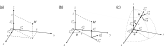
\includegraphics[width=\textwidth]{Chapitre1/Figures/reperes3D.pdf}
	\caption{Systèmes de coordonnées en 3D. (a) cartésiennes (b) cylindriques (c) sphériques.}
	\label{fig:rep3D}
\end{figure}

\subsubsection{Coordonnées cartésiennes}

\paragraph{}Pour se repérer dans l'espace en 3D, la manière la plus simple de faire est d'ajouter un axe $(Oz)$ orthogonal au plan $(xOy)$, dont la direction est donnée par le vecteur directeur $\vv{e_z}$ (voir \autoref{fig:rep3D}-(a)). Dans la base $(\vv{e_x}, \vv{e_y}, \vv{e_z})$, le vecteur position $\vv{OM}$ s'écrit alors simplement :

\begin{equation}
	\vv{OM} = x\vv{e_x} + y\vv{e_y} + z\vv{e_z}
\end{equation}

\noindent et $x$, $y$ et $z$ sont les coordonnées cartésiennes du point $M$.

\subsubsection{Autres systèmes de coordonnées dans l'espace}

\paragraph{}Comme il existe les coordonnées polaires en 2D, il existe des systèmes de coordonnées plus spécifiques que les coordonnées cartésiennes en 3D.

\paragraph{}Les coordonnées cylindriques, représentées sur la \autoref{fig:rep3D}-(b), correspondent à l'ajout d'un repérage via l'axe $(Oz)$ en plus des coordonnées polaires dans le plan $(xOy)$. Elles sont particulièrement utiles pour décrire le mouvement le long d'un tube, comme la marche de la kinésine le long d'un microtubule.

\paragraph{}Les coordonnées sphériques, représentées sur la \autoref{fig:rep3D}-(c), correspondent à l'ajout d'un repérage via un second angle $\phi$ en plus des coordonnées polaires. Elles sont particulièrement utiles pour décrire le mouvement sur une sphère, comme le mouvement des humains sur la Terre.

\paragraph{}\textit{Nous savons maintenant comment repérer un point dans l'espace, quelque soit la dimension considérée. Cependant, pour faire de la mécanique, ce qui nous intéresse n'est pas la position fixe d'un objet mais plutôt son évolution au cours du temps. Il va donc falloir ajouter une variable au problème : le temps.}

\section{Notion de référentiel}

\paragraph{}Avant de se lancer dans l'étude générale de l'évolution d'une position au cours du temps, il est utile de rappeler une notion essentielle : celle de référentiel.

\subsection{Problématisation}

\paragraph{}Prenons l'exemple d'une organelle, le noyau par exemple, dans une cellule en migration (voir \autoref{fig:ref}). Du point de vue de la cellule, cette organelle ne bouge pas, elle a une position fixe. Par contre, du point de vue du biologiste en laboratoire, celle-ci se déplace avec la cellule. Cette observation montre que le mouvement d'un objet dépend en fait du point de vue adopté. Il est donc très important de définir au préalable ce point de vue pour caractériser un mouvement et donc lever cette ambiguïté.

\begin{figure}[h]
	\centering
	\includegraphics[width=0.8\textwidth]{Chapitre1/Figures/ref.pdf}
	\caption{Trajectoires du noyau d'une cellule en migration dans deux référentiels différents. Dans le référentiel du laboratoire, le noyau effectue le mouvement de la migration. Dans le référentiel de la cellule, le noyau est immobile.}
	\label{fig:ref}
\end{figure}

\subsection{Définition}

\paragraph{}En physique, on définit rigoureusement le point de vue d'observation à travers la notion de référentiel.

\begin{defi}{Référentiel}
      Le référentiel est le cadre spatio-temporel de l'étude mécanique. Pour le définir on a besoin d'un repère d'espace et d'un repère de temps.
    \end{defi}
    
\paragraph{}Le repère de temps est défini par une origine des temps $t=0$ et une mesure du temps (conventionnellement la seconde). L'origine des temps est arbitraire mais elle doit être fixée en début d'étude afin de pouvoir situer les différents instants sur la flèche du temps.

\paragraph{}Le repère d'espace est défini par une origine des positions (le point $O$), une mesure des distances (conventionnellement le mètre) et trois axes ($(Ox)$, $(Oy)$ et $(Oz)$).

\paragraph{}Dans le cas présenté en problématisation, la différence de mouvement perçu vient du fait que l'origine du repère d'espace est différente selon les points de vue :

\begin{itemize}

	\item Dans le référentiel $\mathcal{R}_c$ de la cellule, l'origine des positions se déplace avec la cellule. Ainsi, l'appareil de Golgi ne se déplace pas dans ce référentiel car sa position par rapport à l'origine du repère d'espace est constante.
	
	\item Dans le référentiel $\mathcal{R}_l$ du laboratoire, l'origine des positions est fixée à la table d'expérimentation. Ainsi, l'appareil de Golgi se déplace dans ce référentiel car sa position par rapport à l'origine du repère d'espace évolue.

\end{itemize}

\paragraph{}In fine, on retiendra qu'il est essentiel de définir le référentiel dans lequel on étudie un mouvement lors de la problématisation d'une situation physique !

\paragraph{}\textit{Une fois le référentiel défini, nous allons voir avec quels outils nous pouvons décrire le mouvement d'un objet, i.e. l'évolution de sa position au cours du temps.}

\section{Les descripteurs du mouvement}

\paragraph{}Dans la suite, on considère le mouvement du point matériel $M$ par rapport à l'origine du repère d'espace $O$, fixe dans le référentiel d'étude $\mathcal{R}$.

\subsection{Le vecteur position}

\subsubsection{Définitions}

\paragraph{}Le premier descripteur évident du mouvement est le vecteur position $\vv{OM}(t)$ que nous avons déjà rencontré. Simplement, ici, dans le cadre de l'étude d'un mouvement, celui-ci dépend du temps (puisque $M$ se déplace au cours du temps). On a donc :

\begin{equation}
	\vv{OM}(t) = x(t)\vv{e_x} + y(t)\vv{e_y} +z(t)\vv{e_z}
\end{equation}

\noindent Les composantes de ce vecteur, et donc sa norme, sont des distances. Elles s'expriment donc en mètre (\SI{}{\meter}). Ce vecteur permet de définir les notions d'équations horaires et de trajectoire.

\begin{defi}{Trajectoire}
      La trajectoire d'un point $M$ est la courbe décrite par l’extrémité du vecteur position au cours du temps.
    \end{defi}
    
\noindent Par exemple, la trajectoire d'un satellite géostationnaire est un cercle, alors que la trajectoire d'une balle de fusil est un segment.
    
    \begin{defi}{Équations horaires}
      Les équations horaires correspondent aux équations décrivant l'évolution des coordonnées du point $M$ en fonction du temps.
    \end{defi}
    
\noindent Par exemple, les équations horaires représentant un mouvement à vitesse constante $v_0$ dirigée selon $\vv{e_x}$ sont :

\begin{equation}
\left\{
\begin{aligned}
	x(t) &= x_0 + v_0 t \\
	y(t) &= y_0 \\
	z(t) &= z_0
\end{aligned}
\right.
\end{equation}

\noindent tandis que celles décrivant un mouvement circulaire plan de rayon $R_0$ et de vitesse angulaire $\omega$ sont :

\begin{equation}
\left\{
\begin{aligned}
	r(t) &= R_0 \\
	\theta(t) &= \omega t
\end{aligned}
\right.
\end{equation}

\subsubsection{Vecteur déplacement}

\begin{figure}[h]
	\centering
	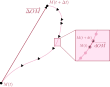
\includegraphics[width=0.5\textwidth]{Chapitre1/Figures/dOM.pdf}
	\caption{Représentation des vecteurs déplacement et déplacement infinitésimal sur une trajectoire}
	\label{fig:dOM}
\end{figure}

\paragraph{}Si l'on considère l'évolution de la position du point $M$ entre l'instant $t$ et l'instant $\Delta t$, il est possible de décrire son déplacement sur la durée $\Delta t$ via le vecteur déplacement :

\begin{equation}
	\vv{\Delta OM}(t) = \vv{OM}(t+\Delta t) - \vv{OM}(t) = \vv{M(t)M(t+\Delta t)}
\end{equation}

\noindent Pour décrire le déplacement de $M$ précisément à chaque instant $t$ il faut considérer des durées $\Delta t$ les plus petites possibles. On parle dans ce cas là de durée infinitésimale (pour dire infiniment petites mais non nulles) et on la note $\mathrm{d}t$. Le vecteur déplacement infinitésimal $\mathrm{d}\vv{OM}(t)$ est alors défini comme :

\begin{equation}
	\mathrm{d}\vv{OM}(t) = \vv{M(t)M(t+\mathrm{d} t)} = \lim_{\Delta t \to 0} \vv{\Delta OM}(t)
\end{equation}

\paragraph{}\textit{Par définition, le vecteur déplacement infinitésimal est toujours tangent à la trajectoire (voir \autoref{fig:dOM}).}

\subsection{Le vecteur vitesse}

\subsubsection{Définition}

\paragraph{}Vous avez normalement déjà toustes entendu parler du concept de vitesse. Prenons l'exemple de la kinésine qui se déplace sur les microtubules. Si elle se déplace d'une distance $D$ sur le microtubule au cours d'une durée $\Delta t$, alors celle-ci a une vitesse $v$ telle que :

\begin{equation}
	v = \frac{D}{\Delta t}
	\label{eq:vbb}
\end{equation}

\noindent Cette grandeur physique s'exprime en mètre par seconde (\SI{}{\meter\per\second}), comme on peut le déduire facilement de l'\autoref{eq:vbb}.

\paragraph{}Dans cet exemple, pour être plus précis, la  vitesse $v$ correspond en fait à la moyenne de la vitesse de la kinésine sur le trajet. En effet, si l'on étudie expérimentalement le trajet d'une kinésine, on se rend compte que son déplacement n'est pas du tout uniforme mais se fait plutôt par pas : elle alterne des phases de pause immobile ($v=0$) et des avancées ponctuelles ($v>0$). Pour spécifier cette notion de moyenne sur le trajet, on préférera alors utiliser la notation $\langle v \rangle$.

\paragraph{}On peut en fait généraliser assez simplement cette notion de vitesse dans le cas où le mouvement se fait dans l'espace et non uniquement en ligne droite. C'est le cas pour la kinésine si le microtubule est courbé par exemple. Dans ce cas là, la vitesse moyenne est définie par un vecteur vitesse moyenne $\langle \vv{v} \rangle$. Dans le cas du mouvement d'un point matériel $M$, il est relié au déplacement $\vv{\Delta OM}$ effectué pendant la durée $\Delta t$ considérée selon :

\begin{equation}
	\langle \vv{v} \rangle = \frac{\vv{\Delta OM}}{\Delta t}
\end{equation}

\noindent On retrouve donc exactement la même définition que précédemment mais appliquée au cas des vecteurs.

\paragraph{}Toutefois, la vitesse moyenne est souvent insuffisante pour décrire correctement un mouvement et un même vecteur $\langle \vv{v} \rangle$ peut décrire des trajectoires extrêmement différentes. Pour une description plus fine, il faut en fait connaître la vitesse du point $M$ à chaque instant $t$, en moyennant le moins possible au cours du trajet. Pour ce faire, on considère donc une durée de trajet infinitésimale $\mathrm{d}t$ afin de définir le vecteur vitesse instantané :

\begin{equation}
	\vv{v} = \lim_{\Delta t \to 0}\frac{\vv{\Delta OM}}{\Delta t} =  \frac{\vv{\mathrm{d}OM}}{\mathrm{d}t} 
\end{equation}

\noindent avec $\vv{\mathrm{d}OM}$ le vecteur déplacement infinitésimal. 

\paragraph{}Mathématiquement, on a $\frac{\vv{\mathrm{d}OM}}{\mathrm{d}t} = \lim_{\Delta t \to 0}\frac{\vv{OM}(t+\Delta t)-\vv{OM}(t)}{\Delta t}$ et donc $\vv{v}$ correspond simplement à la dérivée du vecteur position par rapport au temps. Selon ce principe, on utilisera dans la suite la notation $\frac{\mathrm{d}}{\mathrm{d}t}$ comme équivalente à "dérivée par rapport au temps". De plus, par souci de concision on appellera simplement vecteur vitesse le vecteur vitesse instantanée.

\begin{imp}{Vecteur vitesse}

Le vecteur vitesse correspond à la dérivée du vecteur position en fonction du temps :

\begin{equation}
	\vv{v} =  \frac{\vv{\mathrm{d}OM}}{\mathrm{d}t} 
\end{equation}

\noindent Sa norme s'exprime en \SI{}{\meter\per\second}.

\end{imp}

\subsubsection{Dérivation}

\paragraph{}Afin de calculer une vitesse, il est donc essentiel de maîtriser ses dérivées. Les dérivées de fonctions usuelles sont répertoriées dans le \autoref{tab:der}. Si vous n'êtes pas à l'aise avec cet outil, il est conseillé de reprendre vos cours de lycées.

\begin{table*}[h]
\caption{Dérivée des fonctions usuelles}
  \begin{tabularx}{\textwidth}{s|s}
    \hline\hline
      $$x(t)$$ & $$\frac{\mathrm{d}x}{\mathrm{d}t}$$ \\
      \hline
      $$ t $$ & $$ 1 $$\\
      $$ t^2 $$ & $$ 2t $$\\
      $$ t^n $$ & $$ nt^{n-1} $$\\
      $$ e^t $$ & $$ e^t $$\\
      $$ \cos (t) $$ & $$ -\sin (t) $$\\
      $$ \sin (t) $$ & $$ \cos (t) $$\\
    \hline\hline
  \end{tabularx}
  \label{tab:der}
\end{table*}

\begin{table*}[h]
\caption{Règles de dérivation}
  \begin{tabularx}{\textwidth}{s|s}
    \hline\hline
      $$x(t)$$ & $$\frac{\mathrm{d}x}{\mathrm{d}t}$$ \\
      \hline
      $$ x(at), \quad a=\text{cste} $$ & $$ a \frac{\mathrm{d}x}{\mathrm{d}t}$$\\
      $$ x(t)+y(t) $$ & $$ \frac{\mathrm{d}x}{\mathrm{d}t} + \frac{\mathrm{d}y}{\mathrm{d}t} $$\\
      $$ x(t)\times y(t) $$ & $$ \frac{\mathrm{d}x}{\mathrm{d}t}\times y(t) + x(t)\frac{\mathrm{d}y}{\mathrm{d}t} $$\\
      $$ x(y(t)) $$ & $$ \frac{\mathrm{d}y}{\mathrm{d}t}\times \frac{\mathrm{d}x}{\mathrm{d}y} $$\\
    \hline\hline
  \end{tabularx}
\end{table*}

\paragraph{}Dériver un vecteur peut paraître un peu déstabilisant au premier abord mais si l'on connaît ses règles de dérivation, c'est en fait très simple. Dans le cas des coordonnées cartésiennes on a :

\begin{equation}
	\vv{v} = \frac{\vv{\mathrm{d}OM}}{\mathrm{d}t} = \frac{\mathrm{d}}{\mathrm{d}t}\left( x(t)\vv{e_x} + y(t)\vv{e_y} +z(t)\vv{e_z} \right)
\end{equation}

\noindent La base $(\vv{e_x}, \vv{e_y}, \vv{e_z})$ étant fixe, les vecteurs unitaires sont constants au cours du temps. Ainsi on a simplement :

\begin{equation}
	\vv{v} = \frac{\mathrm{d}x}{\mathrm{d}t}\vv{e_x} + \frac{\mathrm{d}y}{\mathrm{d}t}\vv{e_y} + \frac{\mathrm{d}z}{\mathrm{d}t}\vv{e_z}
\end{equation}

\noindent Ainsi les composantes du vecteur vitesse sont simplement les dérivées des composantes du vecteur position.

\begin{exemple}
	Considérons le vecteur position :
	
	\begin{equation}
		\vv{OM}(t) = 3t~\vv{e_x} + e^{-t}~\vv{e_y}
	\end{equation}
	
	\noindent alors le vecteur vitesse associé est :
	
	\begin{equation}
		\vv{v}(t) = 3~\vv{e_x} - e^{-t}~\vv{e_y}
	\end{equation}
	
\end{exemple}

\subsection*{Exemple du mouvement de la kinésine}

\subsection{Le vecteur accélération}

\paragraph{}De la même manière que la vitesse caractérise la variation de la position au cours du temps, l'accélération caractérise la variation de la vitesse au cours du temps. Lorsqu'on accélère on augmente sa vitesse alors que lorsque l'on décélère on diminue sa vitesse. On définit donc de même un vecteur accélération à tout instant $t$.

\begin{imp}{Vecteur accélération}

Le vecteur accélération correspond à la dérivée du vecteur vitesse en fonction du temps et donc à la dérivée double\footnote{On utilisera la notation $\frac{\mathrm{d}^2}{\mathrm{d}t^2}$ pour désigner la dérivée double par rapport au temps.} du vecteur position en fonction du temps :

\begin{equation}
	\vv{a} =  \frac{\vv{\mathrm{d}v}}{\mathrm{d}t} =  \frac{\vv{\mathrm{d}^2OM}}{\mathrm{d}t^2} 
\end{equation}

\noindent Sa norme s'exprime en \SI{}{\meter\per\second\squared}.

\end{imp}

\paragraph{}Si l'on connaît l'expression du vecteur position au cours du temps, on peut donc  caractériser complètement le mouvement en calculant les vecteurs vitesse et accélération associés.

\begin{exemple}
	Considérons le vecteur position :
	
	\begin{equation}
		\vv{OM}(t) = t^2~\vv{e_x} + \cos (t)~\vv{e_y}
	\end{equation}
	
	\noindent alors le vecteur vitesse associé est :
	
	\begin{equation}
		\vv{v}(t) = 2t~\vv{e_x} - \sin (t)~\vv{e_y}
	\end{equation}
	
	\noindent et le vecteur accélération est :
	
	\begin{equation}
		\vv{a}(t) = 2~\vv{e_x} - \cos (t)~\vv{e_y}
	\end{equation}
	
\end{exemple}

\paragraph{}De manière inverse, si l'on connaît l'accélération du point $M$ ou sa vitesse et que l'on veut déterminer son vecteur position il faut faire le chemin inverse, donc non pas dériver mais intégrer. Il ne faut alors pas oublier les constantes d'intégration qui se déduisent des conditions initiales du mouvement (c'est-à-dire les caractéristiques du mouvement $t=0$). Si vous n'êtes pas à l'aise avec la notion d'intégration, il est fortement conseillé de reprendre un cours de mathématique de niveau lycée.

\begin{exemple}
	Considérons une voiture modélisée par un point matériel $M$ se déplaçant en 1D sur un axe $(Ox)$,  ayant une accélération constante :
	
	\begin{equation}
		\vv{a}(t) = F~\vv{e_x}
	\end{equation}
	
	\noindent et ayant comme position initiale $\vv{OM}(t=0) = x_0 \vv{e_x}$ et comme vitesse initiale $\vv{v} = v_0 \vv{e_x}$. On peut calculer le vecteur vitesse par intégration :
	
	\begin{equation}
		\vv{v}(t) = (Ft+C_1)~\vv{e_x}  
	\end{equation}
	
	\noindent or on sait qu'à $t=0$ on a $\vv{v}=\vv{0}$ donc $C_1=0$. On peut alors intégrer une seconde fois pour trouver le vecteur position :
	
	\begin{equation}
		\vv{OM}(t) = \left(\frac{1}{2}Ft^2+C_2\right)~\vv{e_x}  
	\end{equation}
	
	\noindent or on sait qu'à $t=0$ on a $\vv{OM}=x_0\vv{e_x}$ donc $C_2=x_0$. Ainsi on a finalement :
	
	\begin{equation}
		\vv{OM}(t) = \left(\frac{1}{2}Ft^2+x_0\right)~\vv{e_x}  
	\end{equation}
	
\end{exemple}

\section{Étude de mouvements caractéristiques ($\star$)}

\paragraph{}\textit{Pour mettre en pratique tous ces outils nous allons étudier dans cette dernière partie trois mouvements caractéristique simples.}

\subsection{Mouvement rectiligne uniforme}

\paragraph{}Beaucoup de mouvements peuvent être décrits par un vecteur vitesse $\vv{v_0}$ constant au cours du temps. Cela signifie que la norme de la vitesse $v_0$ est constante et que sa direction l'est aussi. On peut par exemple penser au trajet de migration d'une cellule sur un substrat unidimensionnel.

\begin{figure}[h]
	\centering
	\includegraphics[width=0.7\textwidth]{Chapitre1/Figures/MRU.pdf}
	\caption{Description de la trajectoire d'une cellule en migration rectiligne uniforme.}
	\label{fig:MRU}
\end{figure}

\paragraph{}La meilleure manière de représenter un tel trajet est sur une droite. En effet, dans un repère choisi judicieusement, le mouvement se fait selon un axe. Définissons un axe $(Ox)$ de vecteur directeur unitaire $\vv{e_x}$ dans la même direction que $\vv{v_0}$, tel que $\vv{v_0} = v_0\vv{e_x}$ (voir \autoref{fig:MRU}). Dans ce repère, les descripteurs du mouvement prennent la forme :

\begin{equation}
	\vv{OM}(t) = x(t)\vv{e_x}, \quad \vv{v}(t) = v_x(t) \vv{e_x}, \quad \vv{a}(t) = a_x(t) \vv{e_x}
\end{equation}

\paragraph{}On a donc $v_x(t) = v_0$ qui est indépendant du temps. $a_x(t)$ étant la dérivée de $v_x(t)$, celle-ci est nulle et donc on a $a_x(t)=0$. Enfin, pour trouver l'équation horaire $x(t)$, il suffit d'intégrer :

\begin{equation}
	x(t) = v_0 t + C
\end{equation}

\noindent avec $C$ une constante d'intégration à déterminer à l'aide des conditions initiales. En supposant que l'objet est à la position $\vv{OM}(t=0)=x_0$ à l'instant initial, on a alors $C=x_0$. Les trois descripteurs de ce mouvement sont alors :

\begin{equation}
\vv{OM}(t) = v_0 t + x_0, \quad \vv{v}(t)=v_0\vv{e_x}, \quad \vv{a}(t) = \vv{0}
\end{equation}

\subsection{Mouvement uniformément accéléré}

\paragraph{}Certains mouvements peuvent être décrit par un vecteur accélération constant. C'est le cas du mouvement d'une balle soumise à la gravité par exemple. Considérons un objet se déplaçant dans le plan $xOy$ soumis à une accélération constante $\vv{a}(t) = a_y \vv{e_y}$, avec une vitesse initiale $v(t=0) = v_0\vv{e_x}$ et une position initiale $\vv{OM}(t=0) = x_0 \vv{e_x}$. Essayons de déterminer la vitesse et la position de cet objet à tout instant $t$.

\paragraph{}Pour obtenir la vitesse, il suffit d'intégrer l'accélération, sans oublier les constantes d'intégration :

\begin{equation}
	\vv{v}(t) = C_1 \vv{e_x} + (a_y t + C_2) \vv{e_y}
\end{equation}

\noindent On détermine alors ces constantes d'intégration sachant que $v(t=0) = v_0\vv{e_x}$ et donc $v_x(t=0)=v_0$ et $v_y(t=0)=0$. On obtient alors $C_1 = v_0$ et $C_2=0$ soit :

\begin{equation}
	\vv{v}(t) = v_0 \vv{e_x} + a_y t \vv{e_y}
\end{equation}

\paragraph{}Pour obtenir la position, il suffit d'intégrer la vitesse. De même on a :

\begin{equation}
	\vv{OM}(t) = (v_0 t + C_3) \vv{e_x} + \left(\frac{1}{2}a_y t^2 + C_4\right) \vv{e_y}
\end{equation}

\noindent En utilisant les conditions initiales sur la position on trouve finalement $C_3 = x_0$ et $C_4=0$. Finalement, les trois descripteurs de ce mouvements sont donc :

\begin{equation}
	\vv{OM}(t) = (v_0 t + x_0) \vv{e_x} + \frac{1}{2}a_y t^2 \vv{e_y},\quad \vv{v}(t) = v_0 \vv{e_x} + a_y t \vv{e_y}, \quad \vv{a}(t) = a_y \vv{e_y}
\end{equation}

\paragraph{Équation de la trajectoire} En reprenant les équations horaires :

\begin{equation}
	\left\{\begin{aligned}
	x(t) &= v_0 t + x_0 \\
	y(t) &= \frac{1}{2}a_yt^2
	\end{aligned}\right.
\end{equation}

\noindent il est possible de déterminer la trajectoire de notre mouvement dans le plan $xOy$. Pour ce faire, on commence par exprimer le temps $t$ en fonction de la coordonnée $x$ :

\begin{equation}
	t = \frac{x-x_0}{v_0}
\end{equation}

\noindent puis de remplacer le temps $t$ par cette expression dans l'équation horaire sur la coordonnée $y$ :

\begin{equation}
	y(x) = \frac{a_y}{2v_0^2}(x-x_0)^2
\end{equation}

\noindent Dans le plan $xOy$, l'objet parcourt donc une parabole.

\subsection{Mouvement circulaire uniforme ($\star\star$)}

\paragraph{}Un autre type de mouvement caractéristique sont les mouvements circulaires uniformes. C'est le mouvement associé à un satellite géostationnaire par exemple mais ça peut être aussi le mouvement d'une bactérie dans une colonie sous certaines conditions (voir \autoref{fig:bact_circ}). Considérons un tel mouvement dans le plan $xOy$. De manière évidente, les coordonnées les plus adaptées pour décrire ce mouvement sont les coordonnées polaires. En notant $R$ le rayon de la trajectoire et $\omega$ la vitesse angulaire du mouvement on a :

\begin{equation}
	\left\{\begin{aligned}
	r(t) &= R \\
	\theta (t) &= \omega t
	\end{aligned}\right.
\end{equation}

\paragraph{}Le vecteur position s'écrit dans ce cas :

\begin{equation}
	\vv{OM}(t) = R \vv{e_r}
\end{equation}

\noindent On cherche alors à en déduire l'expression du vecteur vitesse et du vecteur accélération. Pour trouver le vecteur vitesse, il faut dériver le vecteur position :

\begin{equation}
	\vv{v}(t) = \frac{\mathrm{d}}{\mathrm{d}t}\left( R \vv{e_r} \right)
\end{equation}

\noindent mais attention ! Comme nous l'avons vu précédemment, la base polaire est une base mobile, c'est-à-dire que les vecteurs unitaires $\vv{e_r}$ et $\vv{e_\theta}$ dépendent de la position du point $M$ et donc du temps. Ainsi, il faut donc aussi dériver le vecteur $\vv{e_r}$ et ne pas le considérer constant comme dans le cas des coordonnées cartésiennes. En fait, et nous ne le démontrerons pas ici, les dérivées en fonction du temps des vecteurs unitaires de la base polaire sont :

\begin{equation}
	\frac{\mathrm{d}\vv{e_r}}{\mathrm{d}t}=\frac{\mathrm{d}\theta}{\mathrm{d}t}\vv{e_\theta}, \quad \frac{\mathrm{d}\vv{e_\theta}}{\mathrm{d}t}=-\frac{\mathrm{d}\theta}{\mathrm{d}t}\vv{e_r}
\end{equation}

\noindent Ainsi, la dérivée du vecteur position donne dans le cas du mouvement circulaire uniforme :

\begin{equation}
	\vv{v} = R\frac{\mathrm{d}\theta}{\mathrm{d}t}\vv{e_\theta}=R\omega\vv{e_\theta}
\end{equation}

\noindent La vitesse de l'objet est donc dans la direction du vecteur unitaire orthoradial $\vv{e_\theta}$ et sa norme est constante.

\paragraph{}En reprenant le même raisonnement pour calculer l'accélération à partir de la vitesse, on trouve :

\begin{equation}
\vv{a}(t) = -R\omega^2\vv{e_r}
\end{equation}

\noindent Ainsi, l'objet est accéléré vers l'origine du repère. Dans le cas du satellite géostationnaire, cela signifie donc qu'il est accéléré, tiré par le centre de la Terre... Cela vient de la force d'attraction gravitationnelle !

\section*{Objectifs de ce chapitre}

\paragraph{}À l'issue de ce chapitre, vous devez :

\begin{itemize}
	\item Savoir repérer un point sur un axe.
	\item Savoir repérer un point dans le plan en coordonnées cartésiennes et polaires.
	\item Savoir repérer un point dans l'espace en coordonnées cartésiennes.
	\item Avoir compris la notion de référentiel d'étude d'un mouvement.
	\item Écrire un vecteur position à partir des coordonnées d'un point.
	\item Calculer un vecteur déplacement.
	\item Calculer une vitesse moyenne et un vecteur vitesse moyenne.
	\item Définir et calculer un vecteur vitesse instantanée à partir d'un vecteur position.
	\item Définir et calculer un vecteur accélération instantanée à partir d'un vecteur position ou d'un vecteur vitesse.
	\item Retrouver un vecteur position à partir d'un vecteur vitesse ou d'un vecteur accélération et de conditions initiales.
	\item Établir l'équation de la trajectoire d'un point à partir d'un vecteur position.
\end{itemize}
